    \section{Modulacja szerokości impulsu - PWM} 
        \subsection{Opis}
            Najpopularniejszym sposobem sterowania silnikami prądu stałego jest wykorzystanie metody PWM \cite{pwm} czyli modulacji szerokości impulsu. Cechuje się ona tym że nie wymaga użycia skomplikowanych przetworników cyfrowo-analogowych, jednocześnie umożliwiając płynne sterowanie mocą elementów takich jak diody czy silniki. Jej działanie polega na bardzo szybkim przełączaniu pomiędzy stanami wysokim i niskim. Im dłuższy okres czasu zajmuje stan wysoki w cyklu pracy regulatora, tym więcej energii dostarczane jest do sterowanego elementu. Stosunek tego okresu do okresu pracy PWM nazywany jest wypełnieniem. Przebiegi przy trzech różnych wypełnieniach zostały przedstawione na obrazku \ref{fig:pwm_duty}.
            
            \vspace{1em}
                                
            \begin{figure}[ht]
                \centering
                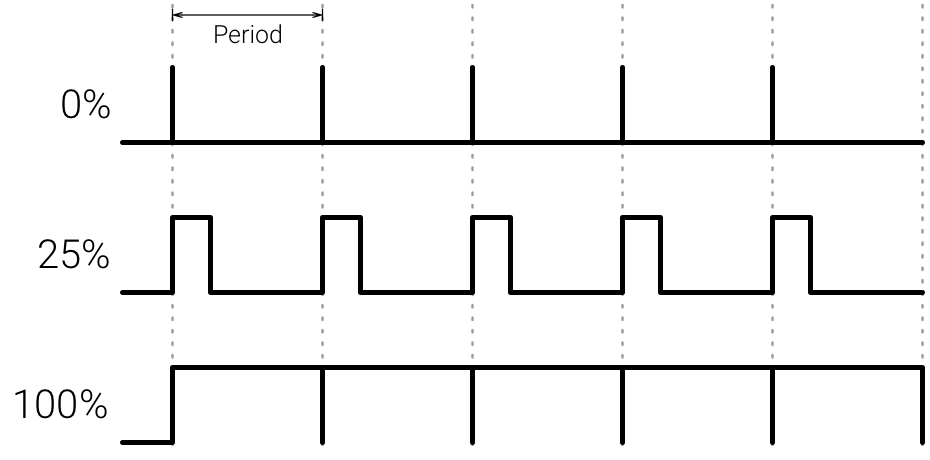
\includegraphics[width=1\textwidth]{img/pwm-duty.png}
                \caption{Przebieg modulacji PWM}
                \label{fig:pwm_duty}
            \end{figure}
            
            \vspace{1em}
        
        
        \subsection{Implementacja}
            Stworzenie obiektu "Motor" automatycznie inicjalizuje peryferium odpowiedzialne na obsługę PWM. Wybór częstotliwości pracy był podyktowany minimalizacją hałasu generowanego podczas pracy silnika. Z tego powodu zdecydowano się na wartość 22kHz, czyli granice ludzkiego słuchu. Jest to także typowa wartość proponowana przez producenta użytego mostka H \cite{mostek}.
            
            Peryferium znajdujące się w wykorzystanym układzie pozwala na generowanie symetrycznego PWM. Różni sie ono od tradycyjnej asymetryczenej regulacji tym że generowane impulsy są zawsze symetryczne względem środka. Zaletą takiego rozwiązania jest generowanie mniejszych harmonicznych w napięciach i prądach wyjściowych oraz lepiej naddaje się ono do sterowania silnikami DC \cite{pwm_center}. Porównanie przebiegów symetrycznego i asymetrycznego PWM zostało umieszczone na obrazku \ref{fig:sym_pwm}
            
            \begin{figure}[ht]
                \centering
                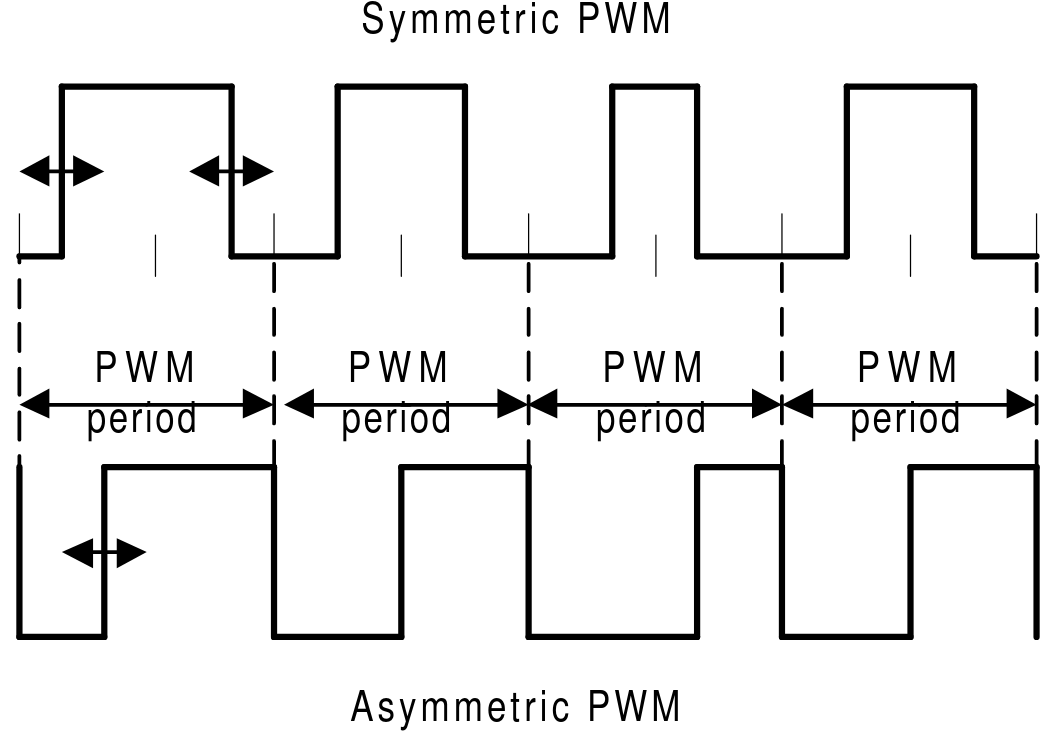
\includegraphics[width=0.9\textwidth]{img/symetric_pwm.png}
                \caption{Przebieg modulacji PWM}
                \label{fig:sym_pwm}
            \end{figure}   
            
            
        \begin{kod}
          \inputminted[firstline=3,lastline=24]{cpp}{esp/listings/motor_driver.cpp}
          \caption{Inicjalizacja PWM}
          \label{code:pwm_init}
          \vspace{2em}
        \end{kod}
        
        Jedyna metoda tej klasy wykorzystywana podczas typowej pracy programu jest przedstawiona na listingu \ref{code:pwm_duty}. Jej zadaniem jest zmiana ustawień wypełnienia PWM oraz kierunku obrotu silnika w zależności od przekazanej wartości.
        
        \begin{kod}
          \inputminted[firstline=27]{cpp}{esp/listings/motor_driver.cpp}
          \caption{Zmiana wypełnienia PWM}
          \label{code:pwm_duty}
          \vspace{2em}
        \end{kod}